\documentclass{CompilerAssignment}
\usepackage{tikz}
\usepackage{subfig}
\usepackage{tabularx}

\usetikzlibrary{arrows,shapes,chains}
\title{Assignment 2}

\newcommand{\eclose}{\epsilon\text{-closure}}
\newcommand{\dtran}{\delta_D}

\begin{document}

\maketitle

\section{Required Exercises}

\subsection{Exercise 1}

\begin{enumerate}
    \item $L\left(\left(\text{a}|\text{b}\right)^*\text{b}\right)$
    
    \begin{figure}[h]
        \centering
        \subfloat[The NFA]{
            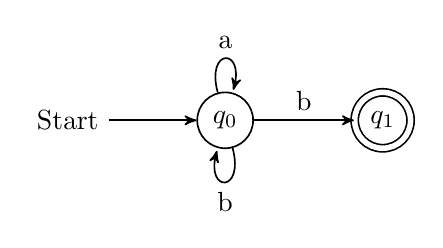
\begin{tikzpicture}[->,>=stealth',auto,semithick]
                \node[style={}](Start)at(-2, 0){Start};
                \node[shape=circle,draw=black](0)at(0, 0){$q_0$};
                \node[shape=circle,draw=black,style=double,double distance=2pt](1)at(2, 0){$q_1$};
                \path[](Start) edge (0)
                (0) edge [loop above] node [above] {a} (0)
                (0) edge [loop below] node [below] {b} (0)
                (0) edge node{b} (1);
            \end{tikzpicture}
        }\qquad
        \subfloat[The DFA]{
            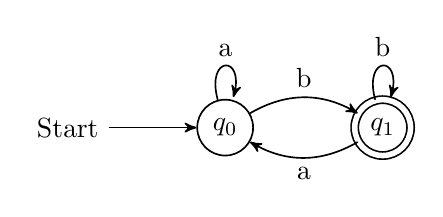
\begin{tikzpicture}[->,>=stealth',auto,semithick]
                \node[style={}](Start)at(-2, 0){Start};
                \node[shape=circle,draw=black](0)at(0, 0){$q_0$};
                \node[shape=circle,draw=black,style=double,double distance=2pt](1)at(2, 0){$q_1$};
                \path[](Start) edge (0)
                (0) edge [loop above] node [above] {a} (0)
                (1) edge [loop above] node [above] {b} (1)
                (0) edge [bend left] node{b} (1)
                (1) edge [bend left] node{a} (0);
            \end{tikzpicture}
        }
    \end{figure}
    
    \item $L\left(\left(\left(\epsilon|\text{a}\right)^*\text{b}\right)^*\right)$
    
    \begin{figure}[h]
        \centering
            \subfloat[The NFA]{
            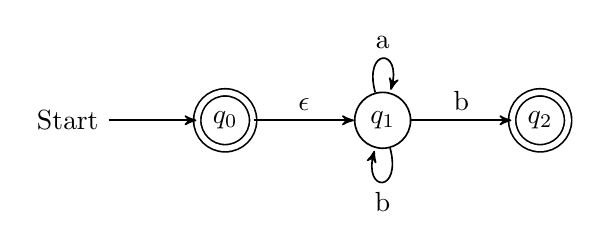
\begin{tikzpicture}[->,>=stealth',auto,semithick]
                \node[style={}](Start)at(-2, 0){Start};
                \node[shape=circle,draw=black,style=double,double distance=2pt](0)at(0, 0){$q_0$};
                \node[shape=circle,draw=black](1)at(2, 0){$q_1$};
                \node[shape=circle,draw=black,style=double,double distance=2pt](2)at(4, 0){$q_2$};
                \path[](Start) edge (0)
                (0) edge node{$\epsilon$} (1)
                (1) edge [loop above] node [above] {a} (1)
                (1) edge [loop below] node [below] {b} (1)
                (1) edge node{b} (2);
            \end{tikzpicture}
        }\qquad
            \subfloat[The DFA]{
            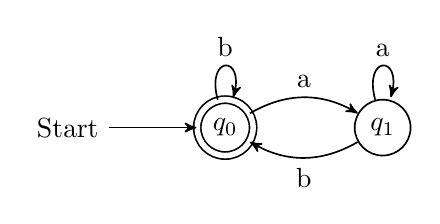
\begin{tikzpicture}[->,>=stealth',auto,semithick]
                \node[style={}](Start)at(-2, 0){Start};
                \node[shape=circle,draw=black,style=double,double distance=2pt](0)at(0, 0){$q_0$};
                \node[shape=circle,draw=black](1)at(2, 0){$q_1$};
                \path[](Start) edge (0)
                (0) edge [loop above] node [above] {b} (0)
                (1) edge [loop above] node [above] {a} (1)
                (0) edge [bend left] node{a} (1)
                (1) edge [bend left] node{b} (0);
            \end{tikzpicture}
            }
    \end{figure}

    \item $L\left(\left(\text{a}|\text{b}\right)^*\text{a}\left(\text{a}|\text{b}\right)\left(\text{a}|\text{b}\right)\right)$
    
    \begin{figure}[h]
        \centering
        \subfloat[The NFA]{
            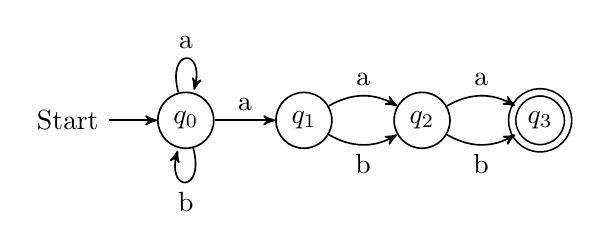
\begin{tikzpicture}[->,>=stealth',auto,semithick]
                \node[style={}](Start)at(-1.5, 0){Start};
                \node[shape=circle,draw=black](0)at(0, 0){$q_0$};
                \node[shape=circle,draw=black](1)at(1.5, 0){$q_1$};
                \node[shape=circle,draw=black](2)at(3, 0){$q_2$};
                \node[shape=circle,draw=black,style=double,double distance=2pt](3)at(4.5, 0){$q_3$};
                \path[](Start) edge (0)
                (0) edge [loop above] node [above] {a} (0)
                (0) edge [loop below] node [below] {b} (0)
                (0) edge node{a} (1)
                (1) edge [bend left] node[above]{a} (2)
                (1) edge [bend right] node[below]{b} (2)
                (2) edge [bend left] node[above]{a} (3)
                (2) edge [bend right] node[below]{b} (3);
            \end{tikzpicture}
        }\hfill
        \subfloat[The DFA]{
            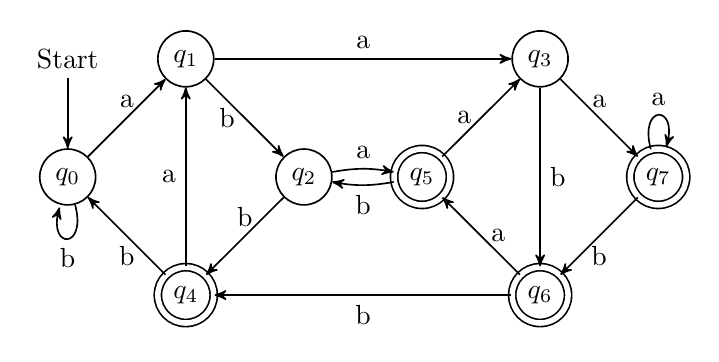
\begin{tikzpicture}[->,>=stealth',auto,semithick]
                \node[style={}](Start)at(0, 1.5){Start};
                \node[shape=circle,draw=black](0)at(0, 0){$q_0$};
                \node[shape=circle,draw=black](1)at(1.5, 1.5){$q_1$};
                \node[shape=circle,draw=black](3)at(6, 1.5){$q_3$};
                \node[shape=circle,draw=black,style=double,double distance=2pt](7)at(7.5, 0){$q_7$};
                \node[shape=circle,draw=black,style=double,double distance=2pt](4)at(1.5, -1.5){$q_4$};
                \node[shape=circle,draw=black](2)at(3, 0){$q_2$};
                \node[shape=circle,draw=black,style=double,double distance=2pt](5)at(4.5, 0){$q_5$};
                \node[shape=circle,draw=black,style=double,double distance=2pt](6)at(6, -1.5){$q_6$};
                \path[](Start) edge (0)
                (0) edge[loop below] node{b} (0)
                (0) edge node[above]{a} (1)
                (1) edge node[left]{b} (2)
                (1) edge node{a} (3)
                (2) edge node[above]{b} (4)
                (2) edge[bend left=10] node{a} (5)
                (3) edge node{b} (6)
                (3) edge node[above]{a} (7)
                (4) edge node[below]{b} (0)
                (4) edge node{a} (1)
                (5) edge[bend left=10] node{b} (2)
                (5) edge node[left]{a} (3)
                (6) edge node{b} (4)
                (6) edge node[right]{a} (5)
                (7) edge node[below]{b} (6)
                (7) edge[loop above] node{a} (7);
            \end{tikzpicture}
        }
    \end{figure}

    \newpage

    \item $L\left(\text{a}^*\text{b}\text{a}^*\text{b}\text{a}^*\text{b}\text{a}^*\right)$
    
    \begin{figure}[h]
        \centering
        \subfloat[The NFA]{
            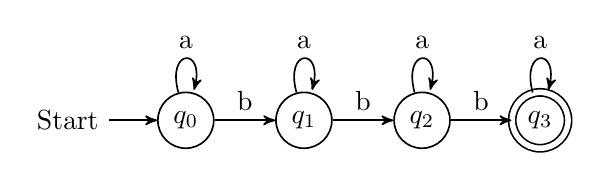
\begin{tikzpicture}[->,>=stealth',auto,semithick]
                \node[style={}](Start)at(-1.5, 0){Start};
                \node[shape=circle,draw=black](0)at(0, 0){$q_0$};
                \node[shape=circle,draw=black](1)at(1.5, 0){$q_1$};
                \node[shape=circle,draw=black](2)at(3, 0){$q_2$};
                \node[shape=circle,draw=black,style=double,double distance=2pt](3)at(4.5, 0){$q_3$};
                \path[](Start) edge (0)
                (0) edge [loop above] node [above] {a} (0)
                (0) edge node{b} (1)
                (1) edge [loop above] node [above] {a} (1)
                (1) edge node{b} (2)
                (2) edge [loop above] node [above] {a} (2)
                (2) edge node{b} (3)
                (3) edge [loop above] node [above] {a} (3);
            \end{tikzpicture}
        }\qquad
        \subfloat[The DFA]{
            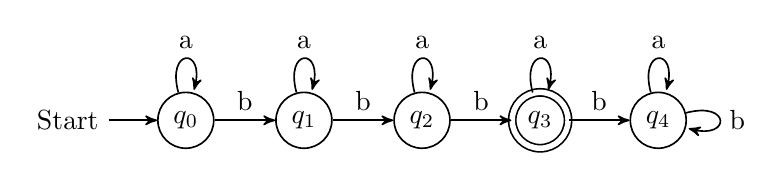
\begin{tikzpicture}[->,>=stealth',auto,semithick]
                \node[style={}](Start)at(-1.5, 0){Start};
                \node[shape=circle,draw=black](0)at(0, 0){$q_0$};
                \node[shape=circle,draw=black](1)at(1.5, 0){$q_1$};
                \node[shape=circle,draw=black](2)at(3, 0){$q_2$};
                \node[shape=circle,draw=black,style=double,double distance=2pt](3)at(4.5, 0){$q_3$};
                \node[shape=circle,draw=black](4)at(6, 0){$q_4$};
                \path[](Start) edge (0)
                (0) edge [loop above] node [above] {a} (0)
                (0) edge node{b} (1)
                (1) edge [loop above] node [above] {a} (1)
                (1) edge node{b} (2)
                (2) edge [loop above] node [above] {a} (2)
                (2) edge node{b} (3)
                (3) edge [loop above] node [above] {a} (3)
                (3) edge node{b} (4)
                (4) edge [loop above] node [above] {a} (4)
                (4) edge [loop right] node [right] {b} (4);
            \end{tikzpicture}
        }
    \end{figure}
\end{enumerate}

\subsection{Exercise 2}

\begin{enumerate}
    \item $\left(\left(\epsilon|\text{a}\right)^*\text{b}\right)^*$
    
    \begin{enumerate}
        \item Construct the NFA for $R_1 = \epsilon|\text{a}$.
        
        \begin{center}
            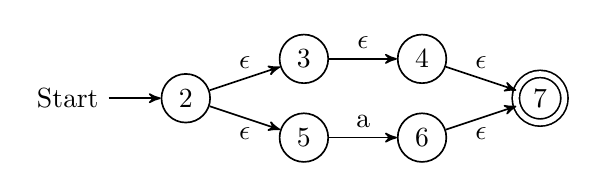
\begin{tikzpicture}[->,>=stealth',auto,semithick]
                \node[style={}](Start)at(1.5, 0){Start};
                % \node[shape=circle,draw=black](0)at(0, 0){$0$};
                % \node[shape=circle,draw=black](1)at(1.5, 0){$1$};
                \node[shape=circle,draw=black](2)at(3, 0){$2$};
                \node[shape=circle,draw=black](3)at(4.5, 0.5){$3$};
                \node[shape=circle,draw=black](4)at(6, 0.5){$4$};
                \node[shape=circle,draw=black](5)at(4.5, -0.5){$5$};
                \node[shape=circle,draw=black](6)at(6, -0.5){$6$};
                \node[shape=circle,draw=black,style=double,double distance=2pt](7)at(7.5, 0){$7$};
                % \node[shape=circle,draw=black](8)at(9, 0){$8$};
                % \node[shape=circle,draw=black](9)at(10.5, 0){$9$};
                % \node[shape=circle,draw=black,style=double,double distance=2pt](10)at(12, 0){$10$};
                \path[](Start) edge (2)
                % (0) edge node{$\epsilon$} (1)
                % (1) edge node{$\epsilon$} (2)
                (2) edge node[above]{$\epsilon$} (3)
                (2) edge node[below]{$\epsilon$} (5)
                (3) edge node{$\epsilon$} (4)
                (5) edge node{a} (6)
                (4) edge node[above]{$\epsilon$} (7)
                (6) edge node[below]{$\epsilon$} (7);
                % (7) edge[bend right=60] node[above]{$\epsilon$} (2)
                % (1) edge[bend right=30] node[below]{$\epsilon$} (8)
                % (7) edge node{$\epsilon$} (8)
                % (8) edge node{b} (9)
                % (9) edge node{$\epsilon$} (10)
                % (9) edge[bend right=50] node[above]{$\epsilon$} (1)
                % (0) edge[bend right=30] node[below]{$\epsilon$} (10);
            \end{tikzpicture}
        \end{center}
        
        \item Construct the NFA for $R_2=\left(\epsilon|\text{a}\right)^*=R_1^*$.
        
        \begin{center}
            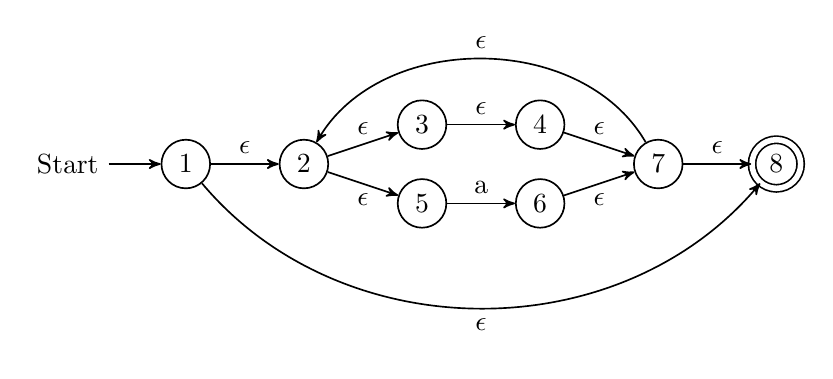
\begin{tikzpicture}[->,>=stealth',auto,semithick]
                \node[style={}](Start)at(0, 0){Start};
                % \node[shape=circle,draw=black](0)at(0, 0){$0$};
                \node[shape=circle,draw=black](1)at(1.5, 0){$1$};
                \node[shape=circle,draw=black](2)at(3, 0){$2$};
                \node[shape=circle,draw=black](3)at(4.5, 0.5){$3$};
                \node[shape=circle,draw=black](4)at(6, 0.5){$4$};
                \node[shape=circle,draw=black](5)at(4.5, -0.5){$5$};
                \node[shape=circle,draw=black](6)at(6, -0.5){$6$};
                \node[shape=circle,draw=black](7)at(7.5, 0){$7$};
                \node[shape=circle,draw=black,style=double,double distance=2pt](8)at(9, 0){$8$};
                % \node[shape=circle,draw=black](9)at(10.5, 0){$9$};
                % \node[shape=circle,draw=black,style=double,double distance=2pt](10)at(12, 0){$10$};
                \path[](Start) edge (1)
                % (0) edge node{$\epsilon$} (1)
                (1) edge node{$\epsilon$} (2)
                (2) edge node[above]{$\epsilon$} (3)
                (2) edge node[below]{$\epsilon$} (5)
                (3) edge node{$\epsilon$} (4)
                (5) edge node{a} (6)
                (4) edge node[above]{$\epsilon$} (7)
                (6) edge node[below]{$\epsilon$} (7)
                (7) edge[bend right=60] node[above]{$\epsilon$} (2)
                (1) edge[bend right=50] node[below]{$\epsilon$} (8)
                (7) edge node{$\epsilon$} (8);
                % (8) edge node{b} (9)
                % (9) edge node{$\epsilon$} (10)
                % (9) edge[bend right=50] node[above]{$\epsilon$} (1)
                % (0) edge[bend right=30] node[below]{$\epsilon$} (10);
            \end{tikzpicture}
        \end{center}

        \item Construct the NFA for $R_3=\left(\epsilon|\text{a}\right)^*\text{b}=R_2\text{b}$.
        
        \begin{center}
            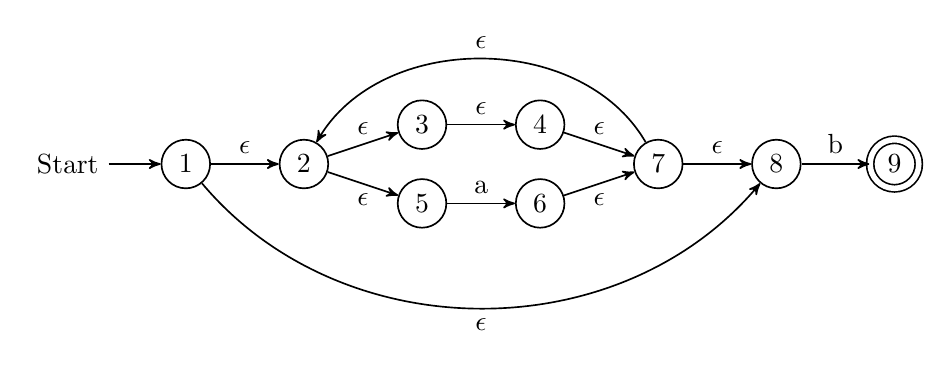
\begin{tikzpicture}[->,>=stealth',auto,semithick]
                \node[style={}](Start)at(0, 0){Start};
                % \node[shape=circle,draw=black](0)at(0, 0){$0$};
                \node[shape=circle,draw=black](1)at(1.5, 0){$1$};
                \node[shape=circle,draw=black](2)at(3, 0){$2$};
                \node[shape=circle,draw=black](3)at(4.5, 0.5){$3$};
                \node[shape=circle,draw=black](4)at(6, 0.5){$4$};
                \node[shape=circle,draw=black](5)at(4.5, -0.5){$5$};
                \node[shape=circle,draw=black](6)at(6, -0.5){$6$};
                \node[shape=circle,draw=black](7)at(7.5, 0){$7$};
                \node[shape=circle,draw=black](8)at(9, 0){$8$};
                \node[shape=circle,draw=black,style=double,double distance=2pt](9)at(10.5, 0){$9$};
                % \node[shape=circle,draw=black,style=double,double distance=2pt](10)at(12, 0){$10$};
                \path[](Start) edge (1)
                % (0) edge node{$\epsilon$} (1)
                (1) edge node{$\epsilon$} (2)
                (2) edge node[above]{$\epsilon$} (3)
                (2) edge node[below]{$\epsilon$} (5)
                (3) edge node{$\epsilon$} (4)
                (5) edge node{a} (6)
                (4) edge node[above]{$\epsilon$} (7)
                (6) edge node[below]{$\epsilon$} (7)
                (7) edge[bend right=60] node[above]{$\epsilon$} (2)
                (1) edge[bend right=50] node[below]{$\epsilon$} (8)
                (7) edge node{$\epsilon$} (8)
                (8) edge node{b} (9);
                % (9) edge node{$\epsilon$} (10)
                % (9) edge[bend right=50] node[above]{$\epsilon$} (1)
                % (0) edge[bend right=30] node[below]{$\epsilon$} (10);
            \end{tikzpicture}
        \end{center}

        \newpage

        \item Construct the NFA for $\left(\left(\epsilon|\text{a}\right)^*\text{b}\right)^*=R_3^*$.

        \begin{center}
            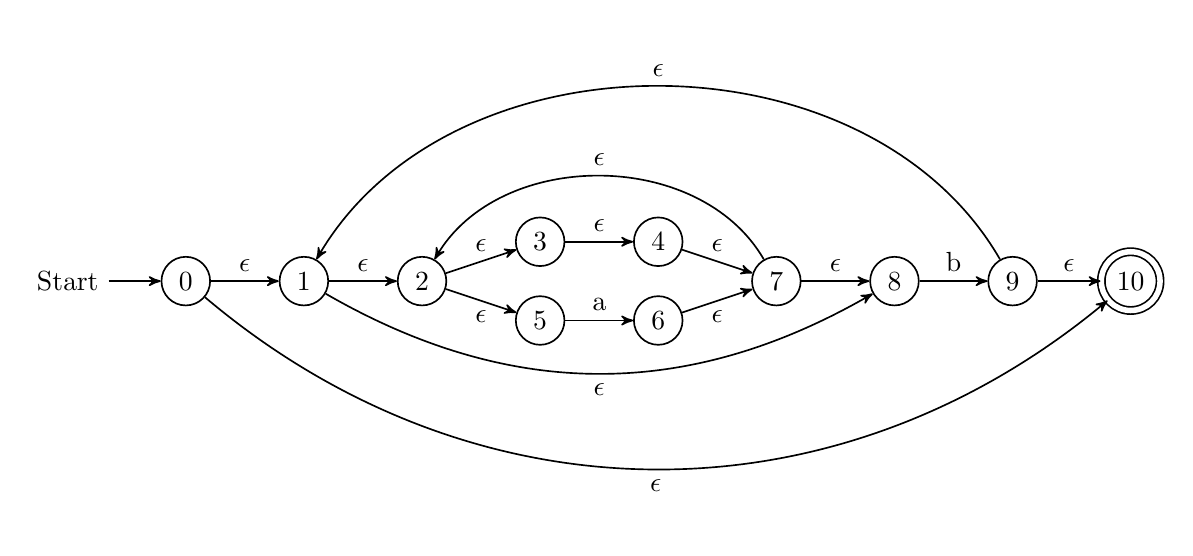
\begin{tikzpicture}[->,>=stealth',auto,semithick]
                \node[style={}](Start)at(-1.5, 0){Start};
                \node[shape=circle,draw=black](0)at(0, 0){$0$};
                \node[shape=circle,draw=black](1)at(1.5, 0){$1$};
                \node[shape=circle,draw=black](2)at(3, 0){$2$};
                \node[shape=circle,draw=black](3)at(4.5, 0.5){$3$};
                \node[shape=circle,draw=black](4)at(6, 0.5){$4$};
                \node[shape=circle,draw=black](5)at(4.5, -0.5){$5$};
                \node[shape=circle,draw=black](6)at(6, -0.5){$6$};
                \node[shape=circle,draw=black](7)at(7.5, 0){$7$};
                \node[shape=circle,draw=black](8)at(9, 0){$8$};
                \node[shape=circle,draw=black](9)at(10.5, 0){$9$};
                \node[shape=circle,draw=black,style=double,double distance=2pt](10)at(12, 0){$10$};
                \path[](Start) edge (0)
                (0) edge node{$\epsilon$} (1)
                (1) edge node{$\epsilon$} (2)
                (2) edge node[above]{$\epsilon$} (3)
                (2) edge node[below]{$\epsilon$} (5)
                (3) edge node{$\epsilon$} (4)
                (5) edge node{a} (6)
                (4) edge node[above]{$\epsilon$} (7)
                (6) edge node[below]{$\epsilon$} (7)
                (7) edge[bend right=60] node[above]{$\epsilon$} (2)
                (1) edge[bend right=30] node[below]{$\epsilon$} (8)
                (7) edge node{$\epsilon$} (8)
                (8) edge node{b} (9)
                (9) edge node{$\epsilon$} (10)
                (9) edge[bend right=60] node[above]{$\epsilon$} (1)
                (0) edge[bend right=40] node[below]{$\epsilon$} (10);
            \end{tikzpicture}
        \end{center}
    \end{enumerate}

    \item $\left(\text{a}|\text{b}\right)^*\text{a}\left(\text{a}|\text{b}\right)\left(\text{a}|\text{b}\right)$
    
    \begin{enumerate}
        \item Construct the NFA for $R_1 = \text{a}|\text{b}$.
        
        \begin{center}
            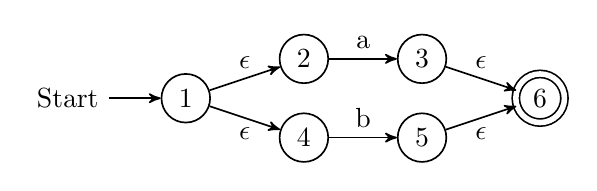
\begin{tikzpicture}[->,>=stealth',auto,semithick]
                \node[style={}](Start)at(1.5, 0){Start};
                \node[shape=circle,draw=black](2)at(3, 0){$1$};
                \node[shape=circle,draw=black](3)at(4.5, 0.5){$2$};
                \node[shape=circle,draw=black](4)at(6, 0.5){$3$};
                \node[shape=circle,draw=black](5)at(4.5, -0.5){$4$};
                \node[shape=circle,draw=black](6)at(6, -0.5){$5$};
                \node[shape=circle,draw=black,style=double,double distance=2pt](7)at(7.5, 0){$6$};
                \path[](Start) edge (2)
                (2) edge node[above]{$\epsilon$} (3)
                (2) edge node[below]{$\epsilon$} (5)
                (3) edge node{a} (4)
                (5) edge node{b} (6)
                (4) edge node[above]{$\epsilon$} (7)
                (6) edge node[below]{$\epsilon$} (7);
            \end{tikzpicture}
        \end{center}

        \item Construct the NFA for $R_2 = \left(\text{a}|\text{b}\right)^* = R_1^*$.
        
        \begin{center}
            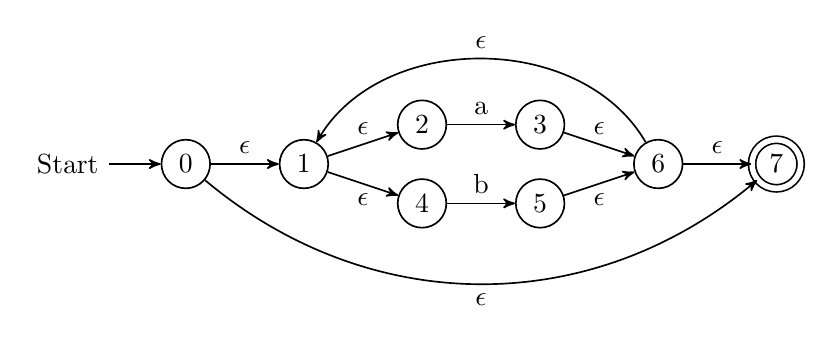
\begin{tikzpicture}[->,>=stealth',auto,semithick]
                \node[style={}](Start)at(0, 0){Start};
                \node[shape=circle,draw=black](1)at(1.5, 0){$0$};
                \node[shape=circle,draw=black](2)at(3, 0){$1$};
                \node[shape=circle,draw=black](3)at(4.5, 0.5){$2$};
                \node[shape=circle,draw=black](4)at(6, 0.5){$3$};
                \node[shape=circle,draw=black](5)at(4.5, -0.5){$4$};
                \node[shape=circle,draw=black](6)at(6, -0.5){$5$};
                \node[shape=circle,draw=black](7)at(7.5, 0){$6$};
                \node[shape=circle,draw=black,style=double,double distance=2pt](8)at(9, 0){$7$};
                \path[](Start) edge (1)
                (1) edge node{$\epsilon$} (2)
                (2) edge node[above]{$\epsilon$} (3)
                (2) edge node[below]{$\epsilon$} (5)
                (3) edge node{a} (4)
                (5) edge node{b} (6)
                (4) edge node[above]{$\epsilon$} (7)
                (6) edge node[below]{$\epsilon$} (7)
                (7) edge[bend right=60] node[above]{$\epsilon$} (2)
                (1) edge[bend right=40] node[below]{$\epsilon$} (8)
                (7) edge node{$\epsilon$} (8);
            \end{tikzpicture}
        \end{center}

        \item Construct the NFA for $R_3 = \left(\text{a}|\text{b}\right)^*\text{a}=R_2\text{a}$.
        
        \begin{center}
            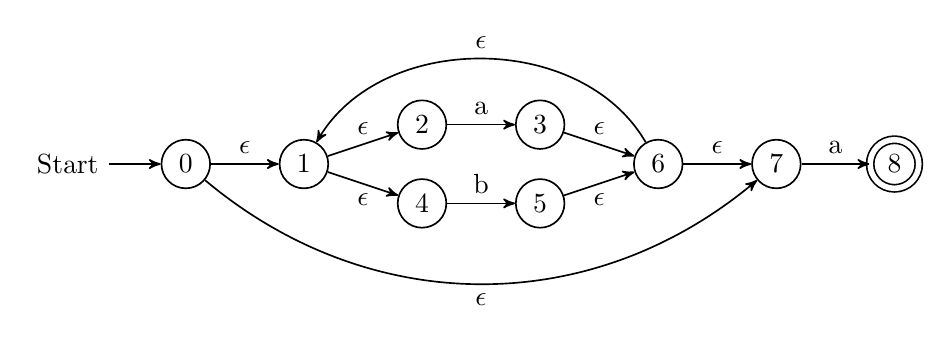
\begin{tikzpicture}[->,>=stealth',auto,semithick]
                \node[style={}](Start)at(0, 0){Start};
                \node[shape=circle,draw=black](1)at(1.5, 0){$0$};
                \node[shape=circle,draw=black](2)at(3, 0){$1$};
                \node[shape=circle,draw=black](3)at(4.5, 0.5){$2$};
                \node[shape=circle,draw=black](4)at(6, 0.5){$3$};
                \node[shape=circle,draw=black](5)at(4.5, -0.5){$4$};
                \node[shape=circle,draw=black](6)at(6, -0.5){$5$};
                \node[shape=circle,draw=black](7)at(7.5, 0){$6$};
                \node[shape=circle,draw=black](8)at(9, 0){$7$};

                \node[shape=circle,draw=black,style=double,double distance=2pt](2_)at(10.5, 0){$8$};
                % \node[shape=circle,draw=black](3_)at(12, .75){$9$};
                % \node[shape=circle,draw=black](4_)at(13.5, .75){$10$};
                % \node[shape=circle,draw=black](5_)at(12, -.75){$11$};
                % \node[shape=circle,draw=black](6_)at(13.5, -.75){$12$};
                % \node[shape=circle,draw=black](7_)at(15, 0){$13$};
                % \node[shape=circle,draw=black](3__)at(16.5, .75){$14$};
                % \node[shape=circle,draw=black](4__)at(18, .75){$15$};
                % \node[shape=circle,draw=black](5__)at(16.5, -.75){$16$};
                % \node[shape=circle,draw=black](6__)at(18, -.75){$17$};
                % \node[shape=circle,draw=black,style=double,double distance=2pt](7__)at(19.5, 0){$18$};
                \path[](Start) edge (1)
                (1) edge node{$\epsilon$} (2)
                (2) edge node[above]{$\epsilon$} (3)
                (2) edge node[below]{$\epsilon$} (5)
                (3) edge node{a} (4)
                (5) edge node{b} (6)
                (4) edge node[above]{$\epsilon$} (7)
                (6) edge node[below]{$\epsilon$} (7)
                (7) edge[bend right=60] node[above]{$\epsilon$} (2)
                (1) edge[bend right=40] node[below]{$\epsilon$} (8)
                (7) edge node{$\epsilon$} (8)
                (8) edge node{a} (2_);
                % \path[]
                % (2_) edge node[above]{$\epsilon$} (3_)
                % (2_) edge node[below]{$\epsilon$} (5_)
                % (3_) edge node{a} (4_)
                % (5_) edge node{b} (6_)
                % (4_) edge node[above]{$\epsilon$} (7_)
                % (6_) edge node[below]{$\epsilon$} (7_);
                % \path[]
                % (7_) edge node[above]{$\epsilon$} (3__)
                % (7_) edge node[below]{$\epsilon$} (5__)
                % (3__) edge node{a} (4__)
                % (5__) edge node{b} (6__)
                % (4__) edge node[above]{$\epsilon$} (7__)
                % (6__) edge node[below]{$\epsilon$} (7__);
            \end{tikzpicture}
        \end{center}

        \newpage

        \item Construct the NFA for $R_4=\left(\text{a}|\text{b}\right)^*\text{a}\left(\text{a}|\text{b}\right)=R_3R_1$.
        
        \begin{center}
            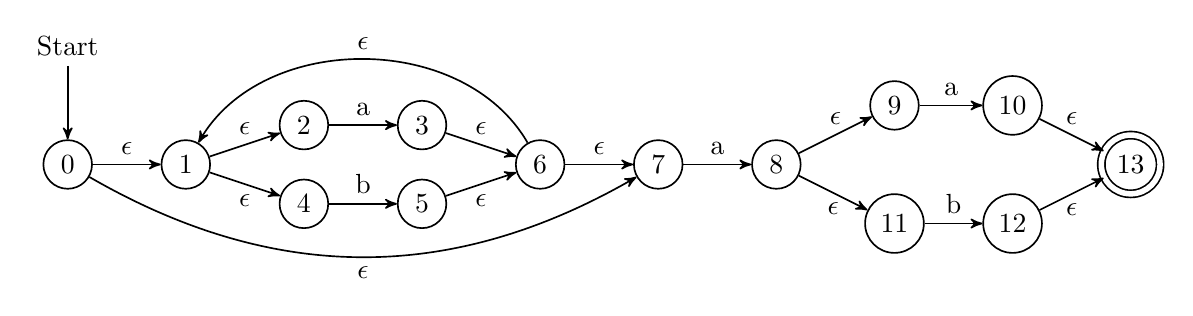
\begin{tikzpicture}[->,>=stealth',auto,semithick]
                \node[style={}](Start)at(1.5, 1.5){Start};
                \node[shape=circle,draw=black](1)at(1.5, 0){$0$};
                \node[shape=circle,draw=black](2)at(3, 0){$1$};
                \node[shape=circle,draw=black](3)at(4.5, 0.5){$2$};
                \node[shape=circle,draw=black](4)at(6, 0.5){$3$};
                \node[shape=circle,draw=black](5)at(4.5, -0.5){$4$};
                \node[shape=circle,draw=black](6)at(6, -0.5){$5$};
                \node[shape=circle,draw=black](7)at(7.5, 0){$6$};
                \node[shape=circle,draw=black](8)at(9, 0){$7$};

                \node[shape=circle,draw=black](2_)at(10.5, 0){$8$};
                \node[shape=circle,draw=black](3_)at(12, .75){$9$};
                \node[shape=circle,draw=black](4_)at(13.5, .75){$10$};
                \node[shape=circle,draw=black](5_)at(12, -.75){$11$};
                \node[shape=circle,draw=black](6_)at(13.5, -.75){$12$};
                \node[shape=circle,draw=black,style=double,double distance=2pt](7_)at(15, 0){$13$};
                % \node[shape=circle,draw=black](3__)at(16.5, .75){$14$};
                % \node[shape=circle,draw=black](4__)at(18, .75){$15$};
                % \node[shape=circle,draw=black](5__)at(16.5, -.75){$16$};
                % \node[shape=circle,draw=black](6__)at(18, -.75){$17$};
                % \node[shape=circle,draw=black,style=double,double distance=2pt](7__)at(19.5, 0){$18$};
                \path[](Start) edge (1)
                (1) edge node{$\epsilon$} (2)
                (2) edge node[above]{$\epsilon$} (3)
                (2) edge node[below]{$\epsilon$} (5)
                (3) edge node{a} (4)
                (5) edge node{b} (6)
                (4) edge node[above]{$\epsilon$} (7)
                (6) edge node[below]{$\epsilon$} (7)
                (7) edge[bend right=60] node[above]{$\epsilon$} (2)
                (1) edge[bend right=30] node[below]{$\epsilon$} (8)
                (7) edge node{$\epsilon$} (8)
                (8) edge node{a} (2_);
                \path[]
                (2_) edge node[above]{$\epsilon$} (3_)
                (2_) edge node[below]{$\epsilon$} (5_)
                (3_) edge node{a} (4_)
                (5_) edge node{b} (6_)
                (4_) edge node[above]{$\epsilon$} (7_)
                (6_) edge node[below]{$\epsilon$} (7_);
                % \path[]
                % (7_) edge node[above]{$\epsilon$} (3__)
                % (7_) edge node[below]{$\epsilon$} (5__)
                % (3__) edge node{a} (4__)
                % (5__) edge node{b} (6__)
                % (4__) edge node[above]{$\epsilon$} (7__)
                % (6__) edge node[below]{$\epsilon$} (7__);
            \end{tikzpicture}
        \end{center}

        \item Construct the NFA for $\left(\text{a}|\text{b}\right)^*\text{a}\left(\text{a}|\text{b}\right)\left(\text{a}|\text{b}\right)=R_4R_1$.
        
        \begin{center}
            \footnotesize
            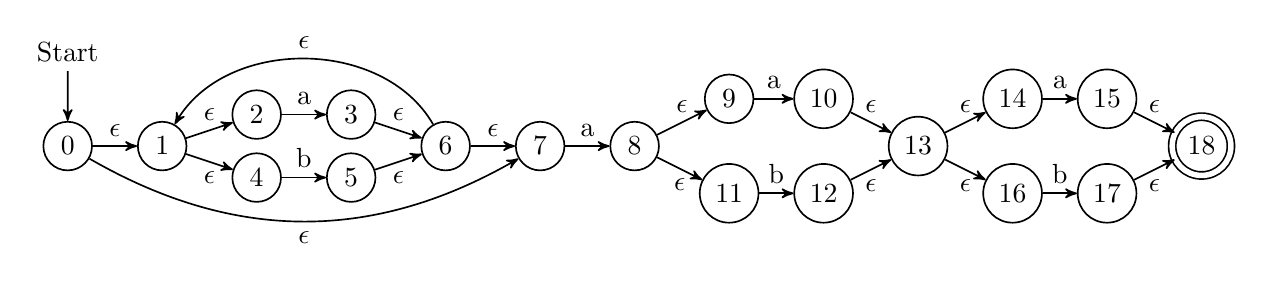
\begin{tikzpicture}[->,>=stealth',auto,semithick,scale=0.8]
                \node[style={}](Start)at(1.5, 1.5){Start};
                \node[shape=circle,draw=black](1)at(1.5, 0){$0$};
                \node[shape=circle,draw=black](2)at(3, 0){$1$};
                \node[shape=circle,draw=black](3)at(4.5, 0.5){$2$};
                \node[shape=circle,draw=black](4)at(6, 0.5){$3$};
                \node[shape=circle,draw=black](5)at(4.5, -0.5){$4$};
                \node[shape=circle,draw=black](6)at(6, -0.5){$5$};
                \node[shape=circle,draw=black](7)at(7.5, 0){$6$};
                \node[shape=circle,draw=black](8)at(9, 0){$7$};

                \node[shape=circle,draw=black](2_)at(10.5, 0){$8$};
                \node[shape=circle,draw=black](3_)at(12, .75){$9$};
                \node[shape=circle,draw=black](4_)at(13.5, .75){$10$};
                \node[shape=circle,draw=black](5_)at(12, -.75){$11$};
                \node[shape=circle,draw=black](6_)at(13.5, -.75){$12$};
                \node[shape=circle,draw=black](7_)at(15, 0){$13$};
                \node[shape=circle,draw=black](3__)at(16.5, .75){$14$};
                \node[shape=circle,draw=black](4__)at(18, .75){$15$};
                \node[shape=circle,draw=black](5__)at(16.5, -.75){$16$};
                \node[shape=circle,draw=black](6__)at(18, -.75){$17$};
                \node[shape=circle,draw=black,style=double,double distance=2pt](7__)at(19.5, 0){$18$};
                \path[](Start) edge (1)
                (1) edge node{$\epsilon$} (2)
                (2) edge node[above]{$\epsilon$} (3)
                (2) edge node[below]{$\epsilon$} (5)
                (3) edge node{a} (4)
                (5) edge node{b} (6)
                (4) edge node[above]{$\epsilon$} (7)
                (6) edge node[below]{$\epsilon$} (7)
                (7) edge[bend right=60] node[above]{$\epsilon$} (2)
                (1) edge[bend right=30] node[below]{$\epsilon$} (8)
                (7) edge node{$\epsilon$} (8)
                (8) edge node{a} (2_);
                \path[]
                (2_) edge node[above]{$\epsilon$} (3_)
                (2_) edge node[below]{$\epsilon$} (5_)
                (3_) edge node{a} (4_)
                (5_) edge node{b} (6_)
                (4_) edge node[above]{$\epsilon$} (7_)
                (6_) edge node[below]{$\epsilon$} (7_);
                \path[]
                (7_) edge node[above]{$\epsilon$} (3__)
                (7_) edge node[below]{$\epsilon$} (5__)
                (3__) edge node{a} (4__)
                (5__) edge node{b} (6__)
                (4__) edge node[above]{$\epsilon$} (7__)
                (6__) edge node[below]{$\epsilon$} (7__);
            \end{tikzpicture}
        \end{center}
    \end{enumerate}

    \item $\text{a}^*\text{b}\text{a}^*\text{b}\text{a}^*\text{b}\text{a}^*$
    
    \begin{enumerate}
        \item Constrcut the NFA for $R_1 = \text{a}^*$.
        
        \begin{center}
            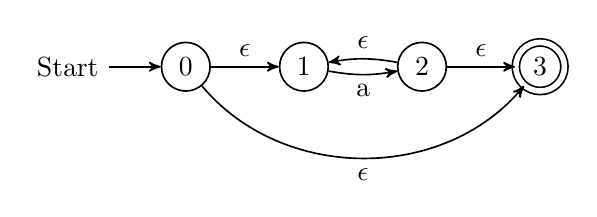
\begin{tikzpicture}[->,>=stealth',auto,semithick]
                \node[style={}](Start)at(-1.5, 0){Start};
                \node[shape=circle,draw=black](0)at(0, 0){$0$};
                \node[shape=circle,draw=black](1)at(1.5, 0){$1$};
                \node[shape=circle,draw=black](2)at(3, 0){$2$};
                \node[shape=circle,draw=black,style=double,double distance=2pt](3)at(4.5, 0){$3$};
                \path[](Start) edge (0)
                (0) edge node{$\epsilon$} (1)
                (1) edge[bend right=10] node[below]{a} (2)
                (2) edge node{$\epsilon$} (3)
                (2) edge[bend right=10] node[above]{$\epsilon$} (1)
                (0) edge[bend right=50] node[below]{$\epsilon$} (3);
            \end{tikzpicture}
        \end{center}

        \item Constrcut the NFA for $R_2 = \text{a}^*\text{b} = R_1\text{b}$.
        
        \begin{center}
            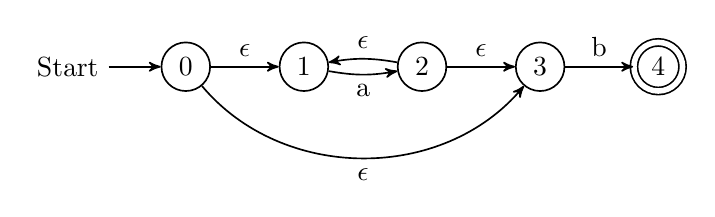
\begin{tikzpicture}[->,>=stealth',auto,semithick]
                \node[style={}](Start)at(-1.5, 0){Start};
                \node[shape=circle,draw=black](0)at(0, 0){$0$};
                \node[shape=circle,draw=black](1)at(1.5, 0){$1$};
                \node[shape=circle,draw=black](2)at(3, 0){$2$};
                \node[shape=circle,draw=black](3)at(4.5, 0){$3$};
                \node[shape=circle,draw=black,style=double,double distance=2pt](4)at(6, 0){$4$};
                \path[](Start) edge (0)
                (0) edge node{$\epsilon$} (1)
                (1) edge[bend right=10] node[below]{a} (2)
                (2) edge node{$\epsilon$} (3)
                (2) edge[bend right=10] node[above]{$\epsilon$} (1)
                (0) edge[bend right=50] node[below]{$\epsilon$} (3);
                \path[] (3) edge node{b} (4);
            \end{tikzpicture}
        \end{center}

        \item Constrcut the NFA for $\text{a}^*\text{b}\text{a}^*\text{b}\text{a}^*\text{b}\text{a}^* = R_2R_2R_2R_1$.
        
        \begin{center}
            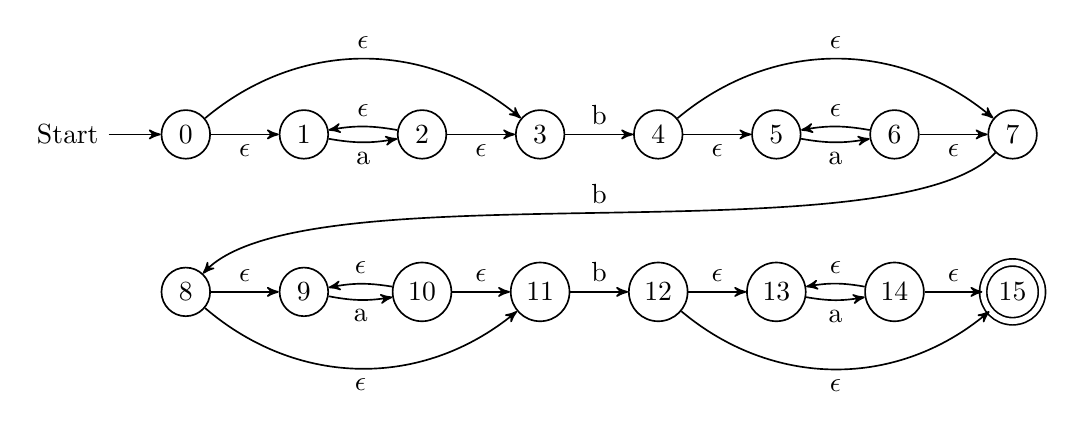
\begin{tikzpicture}[->,>=stealth',auto,semithick]
                \node[style={}](Start)at(-1.5, 0){Start};
                \node[shape=circle,draw=black](0)at(0, 0){$0$};
                \node[shape=circle,draw=black](1)at(1.5, 0){$1$};
                \node[shape=circle,draw=black](2)at(3, 0){$2$};
                \node[shape=circle,draw=black](3)at(4.5, 0){$3$};
                \node[shape=circle,draw=black](4)at(6, 0){$4$};
                \path[](Start) edge (0)
                (0) edge node[below]{$\epsilon$} (1)
                (1) edge[bend right=10] node[below]{a} (2)
                (2) edge node[below]{$\epsilon$} (3)
                (2) edge[bend right=10] node[above]{$\epsilon$} (1)
                (0) edge[bend left=40] node[above]{$\epsilon$} (3);
                \path[] (3) edge node{b} (4);

                \node[shape=circle,draw=black](5)at(7.5, 0){$5$};
                \node[shape=circle,draw=black](6)at(9, 0){$6$};
                \node[shape=circle,draw=black](7)at(10.5, 0){$7$};
                \path[]
                (4) edge node[below]{$\epsilon$} (5)
                (5) edge[bend right=10] node[below]{a} (6)
                (6) edge node[below]{$\epsilon$} (7)
                (6) edge[bend right=10] node[above]{$\epsilon$} (5)
                (4) edge[bend left=40] node[above]{$\epsilon$} (7);

                \node[shape=circle,draw=black](8)at(0, -2){$8$};
                \node[shape=circle,draw=black](9)at(1.5, -2){$9$};
                \node[shape=circle,draw=black](10)at(3, -2){$10$};
                \node[shape=circle,draw=black](11)at(4.5, -2){$11$};
                \node[shape=circle,draw=black](12)at(6, -2){$12$};
                \node[shape=circle,draw=black](13)at(7.5, -2){$13$};
                \node[shape=circle,draw=black](14)at(9, -2){$14$};
                \node[shape=circle,draw=black,style=double,double distance=2pt](15)at(10.5, -2){$15$};
                \draw[] (7) .. controls (9, -1.6) and (1.5, -0.4) .. node[above]{b} (8);
                \path[] (8) edge node{$\epsilon$} (9)
                (9) edge[bend right=10] node[below]{a} (10)
                (10) edge node{$\epsilon$} (11)
                (10) edge[bend right=10] node[above]{$\epsilon$} (9)
                (8) edge[bend right=40] node[below]{$\epsilon$} (11);
                \path[] (11) edge node{b} (12);
                \path[] (12) edge node{$\epsilon$} (13)
                (13) edge[bend right=10] node[below]{a} (14)
                (14) edge node{$\epsilon$} (15)
                (14) edge[bend right=10] node[above]{$\epsilon$} (13)
                (12) edge[bend right=40] node[below]{$\epsilon$} (15);
            \end{tikzpicture}
        \end{center}
    \end{enumerate}
\end{enumerate}

\subsection{Exercise 3}

\begin{enumerate}
    \item
    $A = \eclose(\{0\})=\{0, 1, 2, 3, 4, 5, 7, 8, 10\}.$\\
    $B = \dtran(A, \text{a}) = \eclose(\{6\}) = \{2, 3, 4, 5, 6, 7, 8\}.$\\
    $C = \dtran(A, \text{b}) = \eclose(\{9\}) = \{1, 2, 3, 4, 5, 7, 8, 9, 10\}.$\\
    $D = \dtran(B, \text{a}) = \eclose(\{6\}) = B.$\\
    $E = \dtran(B, \text{b}) = \eclose(\{9\}) = C.$\\
    $F = \dtran(C, \text{a}) = \eclose(\{6\}) = B.$\\
    $G = \dtran(C, \text{b}) = \eclose(\{9\}) = C.$

    Therefore, the transition table of the DFA, whose starting state is $A$ and finite states are $\{A, C\}$, is as follows.

    \begin{center}
        \begin{tabular}{cccc}
            \toprule
            \textsc{NFA State} & \textsc{DFA State} & a & b\\
            \midrule
            \(\{0, 1, 2, 3, 4, 5, 7, 8, 10\}\) & $A$ & $B$ & $C$\\
            \(\{2, 3, 4, 5, 6, 7, 8\}\) & $B$ & $B$ & $C$\\
            \(\{1, 2, 3, 4, 5, 7, 8, 9, 10\}\) & $C$ & $B$ & $C$\\
            \bottomrule
        \end{tabular}
    \end{center}

    Its transition diagram is depicted as follows.

    \begin{center}
        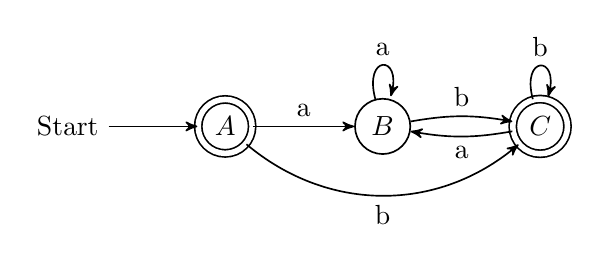
\begin{tikzpicture}[->,>=stealth',auto,semithick]
            \node[style={}](Start)at(-2, 0){Start};
            \node[shape=circle,draw=black,style=double,double distance=2pt](A)at(0, 0){$A$};
            \node[shape=circle,draw=black](B)at(2, 0){$B$};
            \node[shape=circle,draw=black,style=double,double distance=2pt](C)at(4, 0){$C$};
            \path[](Start) edge (A)
            (C) edge [loop above] node [above] {b} (C)
            (B) edge [loop above] node [above] {a} (B)
            (A) edge node{a} (B)
            (C) edge[bend left=10] node{a} (B)
            (A) edge[bend right=40] node[below]{b} (C)
            (B) edge[bend left=10] node{b} (C);
        \end{tikzpicture}
    \end{center}

    \item

    \(A = \eclose(\{0\}) = \{0, 1, 2, 4, 7\}\).\\ %000
    \(B = \dtran(A, \text{a}) = \eclose(\{3, 8\}) = \{1, 2, 3, 4, 6, 7, 8, 9, 11\}\).\\ %001
    \(C = \dtran(A, \text{b}) = \eclose(\{5\}) = \{1, 2, 4, 5, 6, 7\}\).\\ %000
    \(D = \dtran(B, \text{a}) = \eclose(\{3, 8, 10\}) = \{1, 2, 3, 4, 6, 7, 8, 9, 10, 11, 13, 14, 16\}\).\\ %011
    \(E = \dtran(B, \text{b}) = \eclose(\{5, 12\}) = \{1, 2, 4, 5, 6, 7, 12, 13, 14, 16\}\).\\ %010
    \(F = \dtran(C, \text{a}) = \eclose(\{3, 8\}) = B\).\\
    \(G = \dtran(C, \text{b}) = \eclose(\{5\}) = C\).\\
    \(H = \dtran(D, \text{a}) = \eclose(\{3, 8, 10, 15\}) = \{1, 2, 3, 4, 6, 7, 8, 9, 10, 11, 13, 14, 15, 16, 18\}\).\\ %111
    \(I = \dtran(D, \text{b}) = \eclose(\{5, 12, 17\}) = \{1, 2, 4, 5, 6, 7, 12, 13, 14, 16, 17, 18\}\).\\ %110
    \(J = \dtran(E, \text{a}) = \eclose(\{3, 8, 15\}) = \{1, 2, 3, 4, 6, 7, 8, 9, 11, 15, 18\}\).\\ %101
    \(K = \dtran(E, \text{b}) = \eclose(\{5, 17\}) = \{1, 2, 4, 5, 6, 7, 17, 18\}\).\\ %100
    \(L = \dtran(H, \text{a}) = \eclose(\{3, 8, 10, 15\}) = H\).\\
    \(M = \dtran(H, \text{b}) = \eclose(\{5, 12, 17\}) = I\).\\
    \(N = \dtran(I, \text{a}) = \eclose(\{3, 8, 15\}) = J\).\\
    \(O = \dtran(I, \text{b}) = \eclose(\{5, 17\}) = K\).\\
    \(P = \dtran(J, \text{a}) = \eclose(\{3, 8, 10\}) = D\).\\
    \(Q = \dtran(J, \text{b}) = \eclose(\{5, 12\}) = E\).\\
    \(R = \dtran(K, \text{a}) = \eclose(\{3, 8\}) = B\).\\
    \(S = \dtran(K, \text{b}) = \eclose(\{5\}) = C\).

    \newpage

    Therefore, the transition table of the DFA, whose starting state is $A$ and finite states are \(\{H, I, J, K\}\), is as follows.
    
    \begin{center}
        \begin{tabular}{cccc}
            \toprule
            \textsc{NFA State} & \textsc{DFA State} & a & b\\
            \midrule
            \(\{0, 1, 2, 4, 7\}\) & $A$ & $B$ & $C$\\
            \(\{1, 2, 3, 4, 6, 7, 8, 9, 11\}\) & $B$ & $D$ & $E$\\
            \(\{1, 2, 4, 5, 6, 7\}\) & $C$ & $B$ & $C$\\
            \(\{1, 2, 3, 4, 6, 7, 8, 9, 10, 11, 13, 14, 16\}\) & $D$ & $H$ & $I$\\
            \(\{1, 2, 4, 5, 6, 7, 12, 13, 14, 16\}\) & $E$ & $J$ & $K$\\
            \(\{1, 2, 3, 4, 6, 7, 8, 9, 10, 11, 13, 14, 15, 16, 18\}\) & $H$ & $H$ & $I$\\
            \(\{1, 2, 4, 5, 6, 7, 12, 13, 14, 16, 17, 18\}\) & $I$ & $J$ & $K$\\
            \(\{1, 2, 3, 4, 6, 7, 8, 9, 11, 15, 18\}\) & $J$ & $D$ & $E$\\
            \(\{1, 2, 4, 5, 6, 7, 17, 18\}\) & $K$ & $B$ & $C$\\
            \bottomrule
        \end{tabular}
    \end{center}
    
    Its transition diagram is depicted as follows.

    \begin{center}
        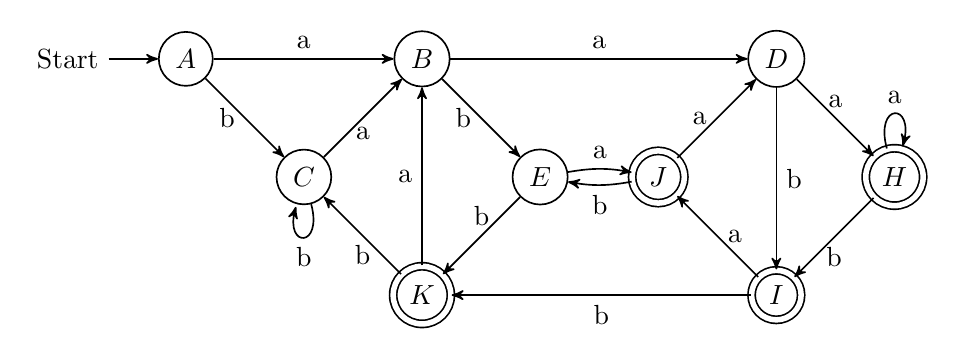
\begin{tikzpicture}[->,>=stealth',auto,semithick]
            \node[style={}](Start)at(-3, 1.5){Start};
            \node[shape=circle,draw=black](S)at(-1.5, 1.5){$A$};
            \node[shape=circle,draw=black](0)at(0, 0){$C$};
            \node[shape=circle,draw=black](1)at(1.5, 1.5){$B$};
            \node[shape=circle,draw=black](3)at(6, 1.5){$D$};
            \node[shape=circle,draw=black,style=double,double distance=2pt](7)at(7.5, 0){$H$};
            \node[shape=circle,draw=black,style=double,double distance=2pt](4)at(1.5, -1.5){$K$};
            \node[shape=circle,draw=black](2)at(3, 0){$E$};
            \node[shape=circle,draw=black,style=double,double distance=2pt](5)at(4.5, 0){$J$};
            \node[shape=circle,draw=black,style=double,double distance=2pt](6)at(6, -1.5){$I$};
            \path[](Start) edge (S)
            (S) edge node[left]{b} (0)
            (S) edge node{a} (1)
            (0) edge[loop below] node{b} (0)
            (0) edge node[below]{a} (1)
            (1) edge node[left]{b} (2)
            (1) edge node{a} (3)
            (2) edge node[above]{b} (4)
            (2) edge[bend left=10] node{a} (5)
            (3) edge node{b} (6)
            (3) edge node[above]{a} (7)
            (4) edge node[below]{b} (0)
            (4) edge node{a} (1)
            (5) edge[bend left=10] node{b} (2)
            (5) edge node[left]{a} (3)
            (6) edge node{b} (4)
            (6) edge node[right]{a} (5)
            (7) edge node[below]{b} (6)
            (7) edge[loop above] node{a} (7);
        \end{tikzpicture}
    \end{center}

    \item 

    $A = \eclose(\{0\}) = \{0, 1, 3\}$.\\
    $B = \dtran(A, \text{a}) = \eclose(\{2\}) = \{1, 2, 3\}$.\\
    $C = \dtran(A, \text{b}) = \eclose(\{4\}) = \{4, 5, 7\}$.\\
    $D = \dtran(B, \text{a}) = \eclose(\{2\}) = B$.\\
    $E = \dtran(B, \text{b}) = \eclose(\{4\}) = C$.\\
    $F = \dtran(C, \text{a}) = \eclose(\{6\}) = \{5, 6, 7\}$.\\
    $G = \dtran(C, \text{b}) = \eclose(\{8\}) = \{8, 9, 11\}$.\\
    $H = \dtran(F, \text{a}) = \eclose(\{6\}) = F$.\\
    $I = \dtran(F, \text{b}) = \eclose(\{8\}) = G$.\\
    $J = \dtran(G, \text{a}) = \eclose(\{10\}) = \{9, 10, 11\}$.\\
    $K = \dtran(G, \text{b}) = \eclose(\{12\}) = \{12, 13, 15\}$.\\
    $L = \dtran(J, \text{a}) = \eclose(\{10\}) = J$.\\
    $M = \dtran(J, \text{b}) = \eclose(\{12\}) = K$.\\
    $N = \dtran(K, \text{a}) = \eclose(\{14\}) = \{13, 14, 15\}$.\\
    $O = \dtran(K, \text{b}) = \emptyset$.\\
    $P = \dtran(N, \text{a}) = \eclose(\{14\}) = N$.\\
    $Q = \dtran(N, \text{b}) = \emptyset = O$.\\
    $R = \dtran(O, \text{a}) = \emptyset = O$.\\
    $S = \dtran(O, \text{b}) = \emptyset = O$.

    Therefore, the transition table of the DFA, whose starting state is $A$ and finite states are \(\{K, N\}\), is as follows.

    \begin{center}
        \begin{tabular}{cccc}
            \toprule
            \textsc{NFA State} & \textsc{DFA State} & a & b\\
            \midrule
            \(\{0, 1, 3\} \) & $A$ & $B$ & $C$\\
            \(\{1, 2, 3\} \) & $B$ & $B$ & $C$\\
            \(\{4, 5, 7\} \) & $C$ & $F$ & $G$\\
            \(\{5, 6, 7\} \) & $F$ & $F$ & $G$\\
            \(\{8, 9, 11\} \) & $G$ & $J$ & $K$\\
            \(\{9, 10, 11\} \) & $J$ & $J$ & $K$\\
            \(\{12, 13, 15\} \) & $K$ & $N$ & $O$\\
            \(\{13, 14, 15\} \) & $N$ & $N$ & $O$\\
            \(\emptyset \) & $O$ & $O$ & $O$\\
            \bottomrule
        \end{tabular}
    \end{center}

    Its transition diagram is depicted as follows.

    \begin{center}
        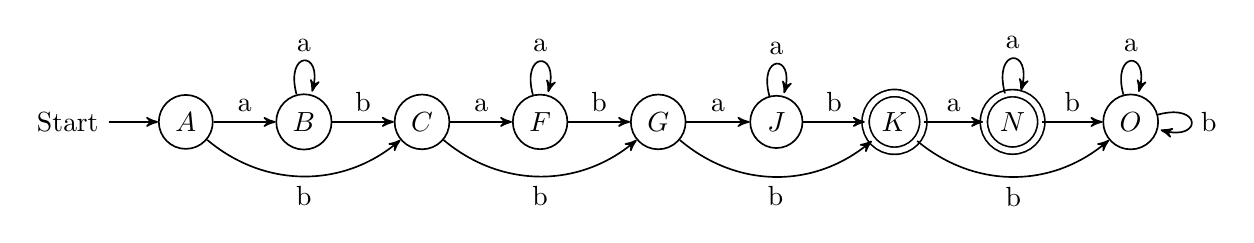
\begin{tikzpicture}[->,>=stealth',auto,semithick]
            \node[style={}](Start)at(-1.5, 0){Start};
            \node[shape=circle,draw=black](A)at(0, 0){$A$};
            \node[shape=circle,draw=black](B)at(1.5, 0){$B$};
            \node[shape=circle,draw=black](C)at(3, 0){$C$};
            \node[shape=circle,draw=black](F)at(4.5, 0){$F$};
            \node[shape=circle,draw=black](G)at(6, 0){$G$};
            \node[shape=circle,draw=black](J)at(7.5, 0){$J$};
            \node[shape=circle,draw=black,style=double,double distance=2pt](K)at(9, 0){$K$};
            \node[shape=circle,draw=black,style=double,double distance=2pt](N)at(10.5, 0){$N$};
            \node[shape=circle,draw=black](O)at(12, 0){$O$};
            \path[](Start) edge (A)
            (A) edge node{a} (B)
            (B) edge node{b} (C)
            (A) edge[bend right=40] node[below]{b} (C)
            (B) edge[loop above] node{a} ()
            (C) edge node{a} (F)
            (F) edge node{b} (G)
            (C) edge[bend right=40] node[below]{b} (G)
            (F) edge[loop above] node{a} ()
            (G) edge node{a} (J)
            (J) edge node{b} (K)
            (G) edge[bend right=40] node[below]{b} (K)
            (J) edge[loop above] node{a} ()
            (K) edge node{a} (N)
            (N) edge node{b} (O)
            (N) edge[loop above] node{a} ()
            (K) edge[bend right=40] node[below]{b} (O)
            (O) edge[loop above] node{a} ()
            (O) edge[loop right] node{b} ();
        \end{tikzpicture}
    \end{center}
\end{enumerate}

\section{Optional Exercises}

\subsection{Exercise 1}

\begin{itemize}
    % \item
    % \begin{enumerate}
    %     \item Initial partition: $G_1 = \{B\}$, $G_2 = \{A, C\}$.
    %     \item Picking $A$, $B$ as the representatives to construct the minimum-state DFA.
    % \end{enumerate}
    % \begin{center}
    %     \begin{tikzpicture}[->,>=stealth',auto,semithick]
    %         \node[style={}](Start)at(-2, 0){Start};
    %         \node[shape=circle,draw=black,style=double,double distance=2pt](0)at(0, 0){$A$};
    %         \node[shape=circle,draw=black](1)at(2, 0){$B$};
    %         \path[](Start) edge (0)
    %         (0) edge [loop above] node [above] {b} (0)
    %         (1) edge [loop above] node [above] {a} (1)
    %         (0) edge [bend left] node{a} (1)
    %         (1) edge [bend left] node{b} (0);
    %     \end{tikzpicture}
    % \end{center}

    \item Regular expression 2:
    
    \begin{enumerate}
        \item Initial partition: $G_1 = \{A, B, C, D, E\}$, $G_2 = \{H, I, J, K\}$.
        \item Handling group $G_1$: b splits it into two groups $G_3 = \{A, B, C, D\}$, $G_4 = \{E\}$.
        \item Handling group $G_3$: a splits it into two groups $G_5 = \{A, B, C\}$, $G_6 = \{D\}$.
        \item Handling group $G_5$: b splits it into two groups $G_7 = \{A, C\}$, $G_8 = \{B\}$.
        \item Handling group $G_2$: a splits it into two groups $G_9 = \{H, I, J\}$, $G_{10} = \{K\}$.
        \item Handling group $G_9$: b splits it into two groups $G_{11} = \{H, J\}$, $G_{12} = \{I\}$.
        \item Handling group $G_{11}$: a splits it into two groups $G_{13} = \{H\}$, $G_{14} = \{J\}$.
        \item Picking $A$, $B$, $D$, $E$, $H$, $I$, $J$, $K$ as the representatives to construct the minimum-state DFA.
    \end{enumerate}
    \begin{center}
        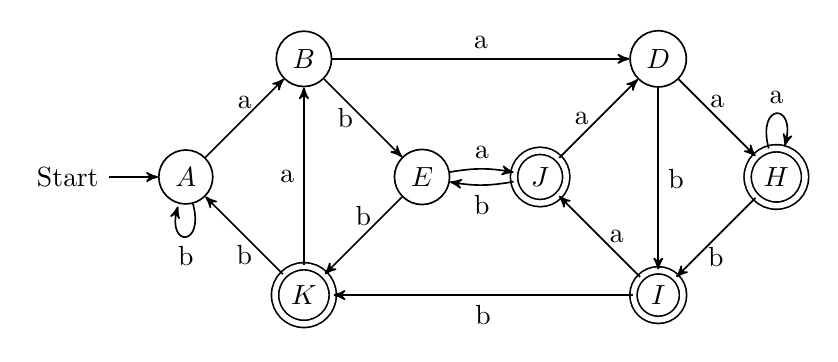
\begin{tikzpicture}[->,>=stealth',auto,semithick]
            \node[style={}](Start)at(-1.5, 0){Start};
            \node[shape=circle,draw=black](0)at(0, 0){$A$};
            \node[shape=circle,draw=black](1)at(1.5, 1.5){$B$};
            \node[shape=circle,draw=black](3)at(6, 1.5){$D$};
            \node[shape=circle,draw=black,style=double,double distance=2pt](7)at(7.5, 0){$H$};
            \node[shape=circle,draw=black,style=double,double distance=2pt](4)at(1.5, -1.5){$K$};
            \node[shape=circle,draw=black](2)at(3, 0){$E$};
            \node[shape=circle,draw=black,style=double,double distance=2pt](5)at(4.5, 0){$J$};
            \node[shape=circle,draw=black,style=double,double distance=2pt](6)at(6, -1.5){$I$};
            \path[](Start) edge (0)
            (0) edge[loop below] node{b} (0)
            (0) edge node[above]{a} (1)
            (1) edge node[left]{b} (2)
            (1) edge node{a} (3)
            (2) edge node[above]{b} (4)
            (2) edge[bend left=10] node{a} (5)
            (3) edge node{b} (6)
            (3) edge node[above]{a} (7)
            (4) edge node[below]{b} (0)
            (4) edge node{a} (1)
            (5) edge[bend left=10] node{b} (2)
            (5) edge node[left]{a} (3)
            (6) edge node{b} (4)
            (6) edge node[right]{a} (5)
            (7) edge node[below]{b} (6)
            (7) edge[loop above] node{a} (7);
        \end{tikzpicture}
    \end{center}

    \item Regular expression 3:
    \begin{enumerate}
        \item Initial partition: $G_1 = \{A, B, C, F, G, J, O\}$, $G_2 = \{K, N\}$.
        \item Handling group $G_1$: a splits it into two groups $G_3 = \{A, B, C, F, O\}$, $G_4 = \{G, J\}$.
        \item Handling group $G_3$: b splits it into two groups $G_5 = \{A, B, O\}$, $G_6 = \{C, F\}$.
        \item Handling group $G_5$: b splits it into two groups $G_7 = \{A, B\}$, $G_8 = \{O\}$.
        \item Picking $A$, $C$, $G$, $K$, $O$ as the representatives to construct the minimum-state DFA.
    \end{enumerate}
    \begin{center}
        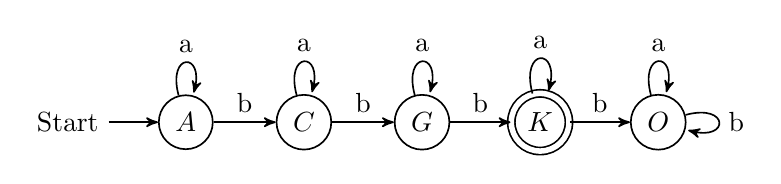
\begin{tikzpicture}[->,>=stealth',auto,semithick]
            \node[style={}](Start)at(-1.5, 0){Start};
            \node[shape=circle,draw=black](0)at(0, 0){$A$};
            \node[shape=circle,draw=black](1)at(1.5, 0){$C$};
            \node[shape=circle,draw=black](2)at(3, 0){$G$};
            \node[shape=circle,draw=black,style=double,double distance=2pt](3)at(4.5, 0){$K$};
            \node[shape=circle,draw=black](4)at(6, 0){$O$};
            \path[](Start) edge (0)
            (0) edge [loop above] node [above] {a} (0)
            (0) edge node{b} (1)
            (1) edge [loop above] node [above] {a} (1)
            (1) edge node{b} (2)
            (2) edge [loop above] node [above] {a} (2)
            (2) edge node{b} (3)
            (3) edge [loop above] node [above] {a} (3)
            (3) edge node{b} (4)
            (4) edge [loop above] node [above] {a} (4)
            (4) edge [loop right] node [right] {b} (4);
        \end{tikzpicture}
    \end{center}
\end{itemize}

\end{document}